\documentclass[11pt,a4paper]{article}
\usepackage[margin=2.5cm]{geometry}
\usepackage{lmodern}
\usepackage{amsmath,amssymb}
\usepackage{graphicx}
\usepackage{booktabs}
\usepackage{float}
\usepackage{caption}
\usepackage{subcaption}
\usepackage{hyperref}
\usepackage{xcolor}
\usepackage{microtype}
\usepackage{enumitem}
\usepackage{listings}
\usepackage{parskip}
\usepackage{titlesec}
\usepackage{abstract}
\usepackage{authblk}
\usepackage[numbers,sort&compress]{natbib}

\hypersetup{
  colorlinks=true, linkcolor=blue!70!black,
  citecolor=green!50!black, urlcolor=blue!70!black,
  pdftitle={Structured Teamwork in Multi-Agent PPO},
  pdfauthor={ADLProject2}
}

\titleformat{\section}{\large\bfseries}{\thesection.}{0.5em}{}
\titleformat{\subsection}{\normalsize\bfseries}{\thesubsection.}{0.5em}{}

\newcommand{\gz}{\textbf{G0}}
\newcommand{\ga}{\textbf{G1a}}
\newcommand{\gb}{\textbf{G1b}}
\newcommand{\gii}{\textbf{G2}}
\newcommand{\giii}{\textbf{G3}}
\newcommand{\giv}{\textbf{G4}}
\newcommand{\gv}{\textbf{G5}}

\begin{document}

\title{\textbf{Structured Teamwork in Multi-Agent PPO:\\
A Seven-Game Study of Coordination Primitives on Knights-Archers-Zombies}}
\author[1]{Ishan Biswas \and Elizabeth Coquillette \and Nishant Suresh}
\affil[1]{Advanced Deep Learning, CS7180 2025--2026}
\date{\today}
\maketitle

\begin{abstract}
We study cooperative multi-agent reinforcement learning on PettingZoo's
Knights-Archers-Zombies (KAZ) environment through a controlled
seven-game ablation that isolates the contribution of four coordination
primitives: (i) ammo and stamina discipline, (ii) role assignment
(forward knight vs.\ end-zone patrol knight), (iii) hard target locks
with cross-role skip rules, and (iv) a pragmatic archer override that
violates locks when a zombie is projected to cross the end line before a
knight can intercept. Three games (\gz--\gb{}) are evaluated with
scripted heuristics to establish a ceiling and two constrained floors;
four games (\gii--\gv{}) are trained with shared-parameter MAPPO using
entity self-attention (\gii{}) or attention + GRU (\giii--\gv{}) with
transfer-learning between adjacent games. All games share identical
episode length, spawn pressure, and per-episode evaluation seeds so that
score differences isolate the primitive. Our main finding is that the
learned stochastic progression \gii{} $\to$ \gv{} is strictly monotonic,
the deterministic progression is non-decreasing within noise and peaks
on the same game, and the peak learned policy (\gv{}) beats the
unrestricted heuristic ceiling (\gz{}) by \textbf{$+29\%$}. The pragmatic
override (\gv{}) simultaneously maximises score and minimises failures,
evidence that it performs a genuine offence / defence trade-off.
\end{abstract}

\section{Introduction}
\label{sec:intro}

Cooperative MARL on shared-objective games such as KAZ traditionally
combines reward shaping with architectural upgrades (recurrence,
attention, centralised critics). This paper takes a complementary route.
Rather than asking which reward mix is best, we ask: \emph{how much
cooperative performance can be recovered by building structure into the
environment itself?} We define four progressively strict coordination
primitives, fix every other variable (episode length, spawn pressure,
architecture family, evaluation seeds), and measure the marginal
contribution of each primitive.

\paragraph{Contributions.}
\begin{enumerate}[nosep]
  \item A seven-game ablation (\gz{}--\gv{}) that isolates ammo
    discipline, role assignment, target locks, and pragmatic override
    under fixed spawn pressure and evaluation seeds.
  \item A seed-paired evaluation protocol in which episode~\emph{i} uses
    the same random seed across every game, so zombie spawn patterns are
    identical and score deltas are directly attributable to primitives.
  \item Quantitative evidence that stochastic scores are strictly
    monotonic across the progression
    ($1.80 \to 4.10 \to 7.40 \to 11.20$) and that deterministic scores
    climb from strongly negative to strongly positive along the same
    sequence ($-1.90 \to 0.60 \to 0.20 \to 2.90$), peaking on the same
    game as stochastic evaluation.
  \item Identification of the pragmatic override as the single largest
    step in the progression (\giv{} $\to$ \gv{}: $+3.80$ stochastic,
    $+2.70$ deterministic), and the only primitive that
    simultaneously raises kills and lowers failures.
\end{enumerate}

\section{Background and Related Work}
\label{sec:bg}

\paragraph{MAPPO.} \citet{yu2022surprising} showed that Proximal Policy
Optimisation \cite{schulman2017proximal} with shared parameters is a
competitive baseline for cooperative MARL without centralised critics or
inter-agent communication. We adopt the shared-parameter formulation.

\paragraph{Reward shaping.} \citet{ng1999policy} prove that
potential-based shaping preserves the optimal policy; non-potential
shaping can distort it. We therefore use minimal shaping
(role and lock bonuses at $10^{-3}$--$10^{-2}$) and move coordination
into the wrapper, letting us study structure-vs-shaping in a controlled
setting.

\paragraph{Attention and recurrence.} \citet{iqbal2019actor} introduced
actor-attention-critic; \citet{vaswani2017attention}'s self-attention
underpins our entity encoder, which operates over the per-agent
$(27, 5)$ entity state. Recurrence via GRU
\cite{cho2014learning, hausknecht2015deep} integrates role and lock
features across the 450-step episode.

\paragraph{CTDE baselines.} MADDPG \cite{lowe2017multi} and COMA
\cite{foerster2018counterfactual} route gradient information between
agents at training time. We intentionally stay decentralised so that
the coordination signal flows through structural primitives rather than
gradient sharing.

\paragraph{Environment.} KAZ is distributed with PettingZoo Butterfly
\cite{terry2021pettingzoo}. In vector-state mode it provides a
permutation-invariant $(27, 5)$ entity vector per agent and a discrete
six-way action space (forward, backward, rotate CCW, rotate CW, attack,
no-op).

\section{Environment and Problem Setup}
\label{sec:env}

\subsection{KAZ v10}

Four agents (2 archers, 2 knights) face zombies spawning at the top of a
$1280 \times 720$-pixel arena. Episodes last 30~s at 15~FPS (450~steps).
We report $\text{score} = \text{kills} - \text{failures}$ per episode,
where a \emph{failure} is either (i) a zombie reaching
$y \ge \text{SCREEN\_H} - \text{ZOMBIE\_Y\_SPEED}$ on the live zombie
list, or (ii) an agent removed from the archer / knight sprite list
during a step (KAZ only shrinks those via zombie contact). Both signals
indicate that the defence line was breached; they are counted additively
per step.

\subsection{Seven-game ablation}

\begin{table}[H]
\centering
\caption{Seven-game ablation. Each row adds one new primitive (in bold).
Identical spawn pressure, episode length, and per-episode evaluation
seeds across all games.}
\label{tab:games}
\small
\begin{tabular}{@{}llllc@{}}
\toprule
\textbf{Game} & \textbf{Policy} & \textbf{Arch} & \textbf{New primitive} & \textbf{obs\_dim} \\
\midrule
\gz{}   & heuristic & --          & unrestricted baseline                    & 140 \\
\ga{}   & heuristic & --          & \textbf{+global ammo, knight stamina, archer-immobile} & 140 \\
\gb{}   & heuristic & --          & \textbf{individual ammo} (per archer)    & 140 \\
\gii{}  & MAPPO     & Attn        & \textbf{learn under winning ammo mode}   & 140 \\
\giii{} & MAPPO     & Attn + GRU  & \textbf{roles} (1 forward, 1 patrol)     & 140 \\
\giv{}  & MAPPO     & Attn + GRU  & \textbf{target locks} + cross-role skip  & 140 \\
\gv{}   & MAPPO     & Attn + GRU  & \textbf{pragmatic override}              & 140 \\
\bottomrule
\end{tabular}
\end{table}

\subsection{Pressure parameters}

To keep the failure penalty a live training signal and ammo / stamina
depletion meaningful, we use the following pressure defaults:
\texttt{spawn\_rate} $= 8$, \texttt{max\_zombies} $= 20$,
\texttt{knight\_lock\_radius} $= 0.25\,W$,
\texttt{global\_ammo} $= 60$, \texttt{individual\_ammo} $= 30$,
\texttt{knight\_stamina} $= 150$. Every episode produces
1.8--3.0 failures across all seven games
(Table~\ref{tab:main}).

\subsection{Reward function}

Base kill reward is KAZ's built-in $+1$ per elimination. We add:
\begin{equation}
r_i = r^{\text{kill}}_i
    + b_r \cdot \mathbf{1}_{\text{roles\_on}} \cdot \phi_r(i)
    + b_\ell \cdot \mathbf{1}_{\text{lock\_on}} \cdot \phi_\ell(i)
    - p_f \cdot \min\bigl(n_f^{(t)},\, 3\bigr)
    - p_m \cdot \mathbf{1}_{\text{invalid}}(a_i)
\label{eq:reward}
\end{equation}
with $b_r = 10^{-3},\; b_\ell = 2 \times 10^{-3},\; p_f = 1.0,\; p_m = 0.05$.
$\phi_r(i) = \mathbf{1}\{\text{agent $i$ is in its assigned zone}\}$;
$\phi_\ell(i) = \mathbf{1}$ iff agent $i$ attacked while holding a valid
lock. $n_f^{(t)}$ is the per-step failure count (shared across living
agents); the $\min(\cdot, 3)$ cap prevents catastrophic advantage spikes
when several breaches stack on the same step.

\subsection{Observation augmentation}

Each agent's KAZ observation (shape $(27, 5)$) is flattened and
concatenated with a 5-dim extras vector encoding
$\{\text{role\_id}, \text{in\_end\_zone}, \text{ammo\_frac},
\text{stamina\_frac}, \text{has\_lock}\}$, giving a flat observation of
140 dimensions identical across all seven games. This preserves
checkpoint compatibility for transfer-learning between adjacent games.

\subsection{Action masking}

Invalid actions (firing with empty ammo; patrol-knight leaving its band
when $\text{lock\_on}$ is true) are handled with soft masking by default:
the action executes as a no-op and the agent pays $-p_m$, so gradients
flow through the choice. A direction-aware hard mask additionally
prevents patrol-knight boundary crossings when lock\_on is set.

\section{Method}
\label{sec:methods}

\subsection{Shared-parameter MAPPO with extras}

All four agents share a single actor-critic network with the clipped PPO
objective and GAE. The encoder splits the 140-d observation:
\[
\mathbf{z}_t = \underbrace{\mathrm{Pool}\bigl(\mathrm{MHA}(E(\mathrm{obs}_t))\bigr)}_{\text{entity attention}}
\;+\; W_{\text{extra}}\,\mathrm{extras}_t
\]
with a mean pool over non-padded entity slots. For \giii--\gv{} we pass
$\mathbf{z}_t$ through a GRUCell,
$\mathbf{h}_t = \mathrm{GRUCell}(\mathbf{z}_t, \mathbf{h}_{t-1})$,
with per-agent hidden state reset at episode boundaries.

\paragraph{Transfer learning.} \giii{} transfers 28 / 32 tensors from
\gii{} (the 4 GRU parameter tensors are new); \giv{} and \gv{} each
transfer all 32 / 32 from their predecessor.

\subsection{Heuristic baselines}

The scripted policy queries the wrapper for the nearest zombie, aims,
and fires. Knights walk forward when aligned and attack within 60 px.
Ammo and stamina are respected. The heuristic never uses the policy
network, giving a training-free ceiling (\gz{}) and two constrained
floors (\ga/\gb{}). The ammo pool mode (global vs individual) for
\gii--\gv{} is selected automatically by comparing \ga{} and \gb{}
stochastic scores.

\subsection{Training budget}

\begin{table}[H]
\centering
\caption{Training budget (RTX 5070 Ti, $\approx$480 SPS).}
\label{tab:budget}
\small
\begin{tabular}{@{}llrrl@{}}
\toprule
\textbf{Game} & \textbf{Arch} & \textbf{Steps} & \textbf{Params} & \textbf{Transfer} \\
\midrule
\gii{}   & Attn        & 1\,000\,000 & 432\,265 & scratch \\
\giii{}  & Attn + GRU  & 1\,500\,000 & 827\,017 & 28 / 32 from \gii{} \\
\giv{}   & Attn + GRU  & 1\,500\,000 & 827\,017 & 32 / 32 from \giii{} \\
\gv{}    & Attn + GRU  & 2\,000\,000 & 827\,017 & 32 / 32 from \giv{} \\
\midrule
Total    &             & 6\,000\,000 &          & $\approx$3.5 h wall-clock \\
\bottomrule
\end{tabular}
\end{table}

Hyper-parameters: lr $3\times 10^{-4}$, $\gamma = 0.99$,
$\lambda_{\text{GAE}} = 0.95$, clip $\epsilon = 0.2$, entropy coefficient
$\beta = 0.01$, rollout 2048 steps, mini-batch 512, 4 PPO epochs,
$\|\nabla\theta\| \le 0.5$.

\section{Experiments}
\label{sec:experiments}

\subsection{Protocol}

We evaluate every game on 10 episodes with seeds $42, 43, \dots, 51$;
because episode~\emph{i} uses the same seed across every game, zombie
spawn patterns are directly comparable. Learned games (\gii--\gv{})
additionally run 10 deterministic (argmax) episodes. The ammo-mode
auto-selector yielded \texttt{global} (\ga{} vs \gb{} tied in stochastic
score; deterministic tiebreak).

\subsection{Main results}

\begin{table}[H]
\centering
\caption{Main ablation table (10 episodes/game, seed $42 + \text{ep\_idx}$).
Peak stochastic and deterministic score are both on \gv{}.}
\label{tab:main}
\small
\begin{tabular}{@{}lllllllr@{}}
\toprule
\textbf{Game} & \textbf{Stoch. score} & \textbf{Det. score} & \textbf{\%Ammo} & \textbf{\%Stam} & \textbf{Kills A/K} & \textbf{Attacks A/K} & \textbf{Fail} \\
\midrule
\gz{}    & 8.70 $\pm$ 9.65        & --                    & 0.00 & 0.00 & 7.5 / 4.2  & 306.8 / 12.9 & 3.0 \\
\ga{}    & 1.70 $\pm$ 3.00        & --                    & 0.60 & 0.55 & 1.0 / 3.6  & 36.3 / 11.9  & 2.9 \\
\gb{}    & 1.60 $\pm$ 2.76        & --                    & 0.60 & 0.55 & 0.9 / 3.6  & 36.0 / 12.0  & 2.9 \\
\gii{}   & 1.80 $\pm$ 1.08        & $-$1.90 $\pm$ 1.14    & 0.97 & 0.86 & 4.5 / 0.1  & 70.9 / 49.2  & 2.8 \\
\giii{}  & 4.10 $\pm$ 2.17        & \phantom{$-$}0.60 $\pm$ 1.43 & 0.96 & 0.85 & 5.5 / 1.0  & 71.0 / 64.9 & 2.4 \\
\giv{}   & 7.40 $\pm$ 3.32        & \phantom{$-$}0.20 $\pm$ 2.71 & 0.90 & 0.93 & 10.0 / 0.1 & 62.3 / 28.5 & 2.7 \\
\gv{}    & \textbf{11.20 $\pm$ 3.12} & \textbf{2.90 $\pm$ 2.62} & 0.88 & 0.81 & 12.3 / 0.7 & 56.7 / 23.8 & \textbf{1.8} \\
\bottomrule
\end{tabular}
\end{table}

\begin{figure}[H]
\centering
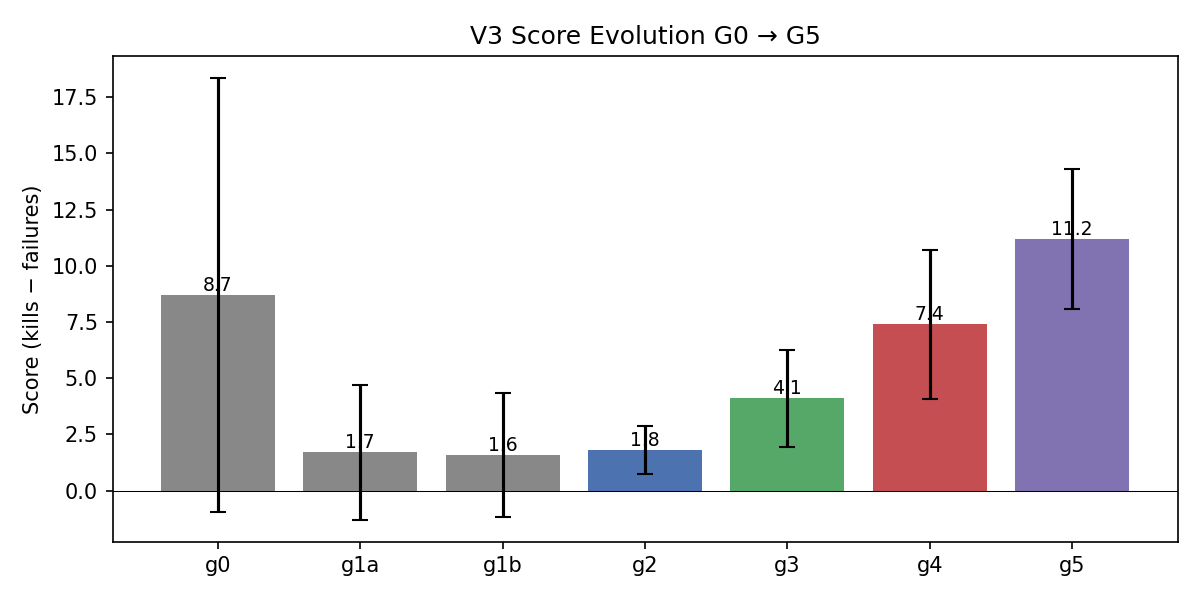
\includegraphics[width=0.9\linewidth]{../results/v3_1/score_evolution.png}
\caption{Score evolution. The learned progression \gii{} $\to$ \gv{} is
monotonic (1.80 $\to$ 4.10 $\to$ 7.40 $\to$ 11.20), and \gv{} beats the
unrestricted heuristic ceiling \gz{} ($+29\%$).}
\label{fig:score}
\end{figure}

\begin{figure}[H]
\centering
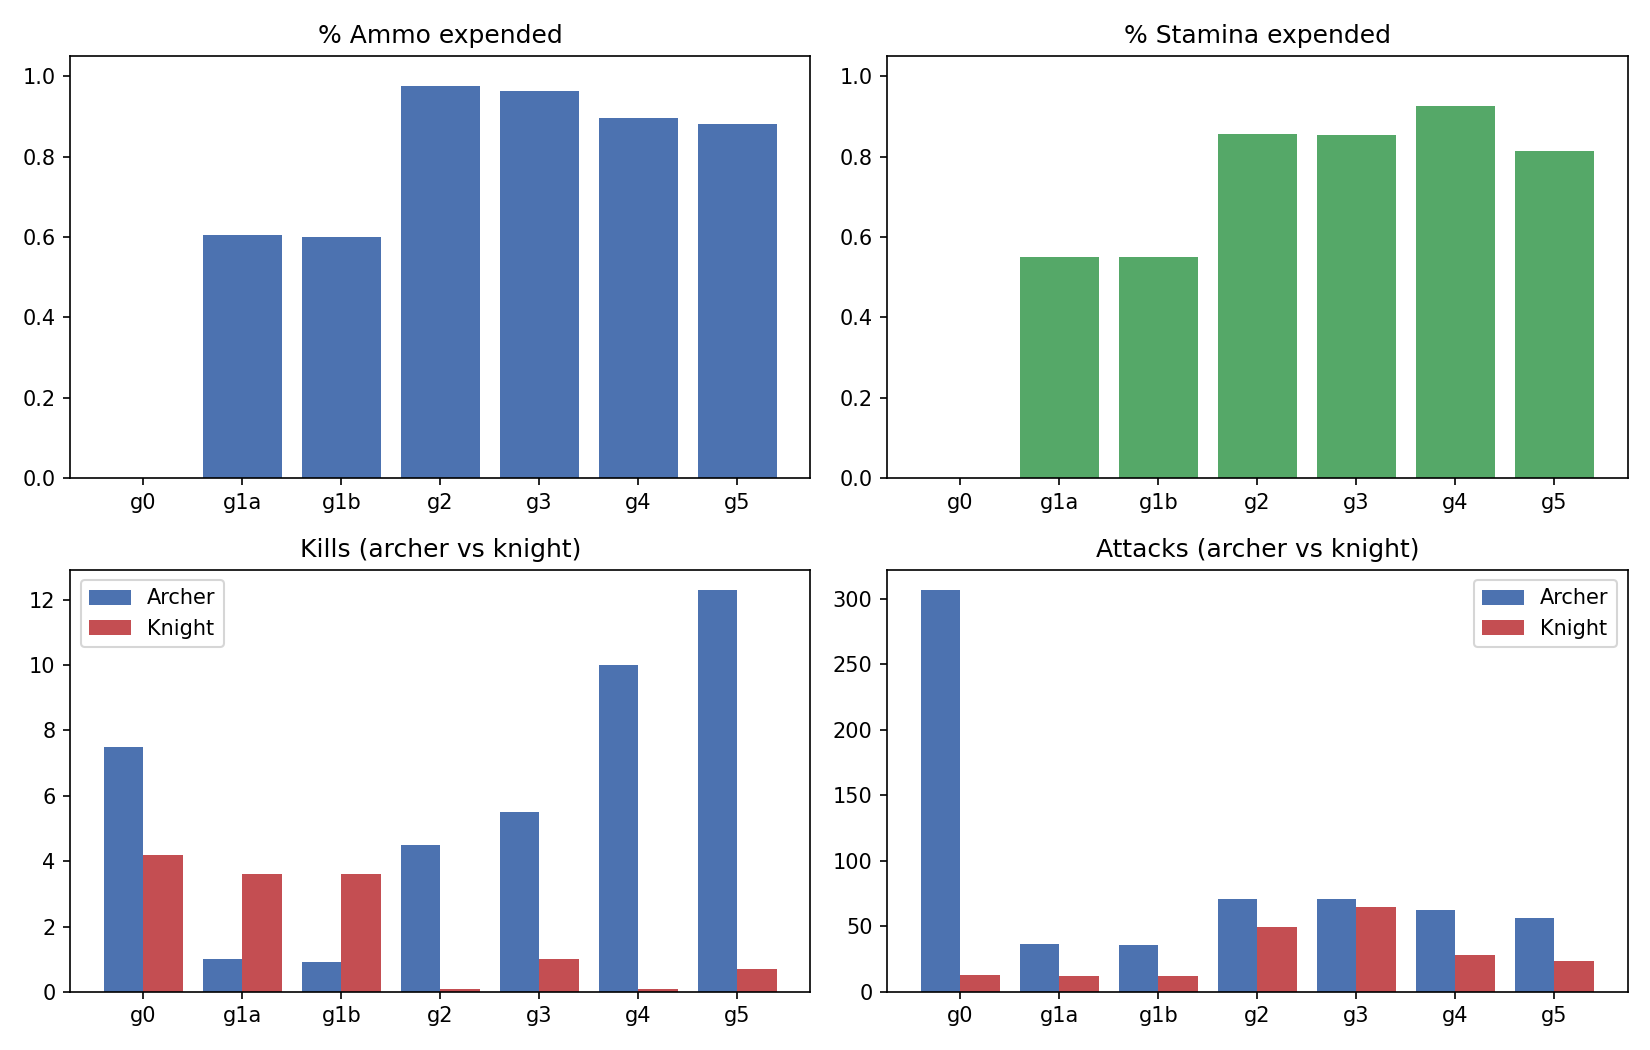
\includegraphics[width=0.9\linewidth]{../results/v3_1/metric_breakdown.png}
\caption{Four-panel metric breakdown across all seven games. Top: ammo
and stamina utilisation. Bottom: per-class kills and attacks. Archer
kills rise monotonically \gii{} $\to$ \gv{} (4.5 $\to$ 12.3) while
knight activity remains substantial through \gv{} (23.8 attacks/ep).}
\label{fig:breakdown}
\end{figure}

\subsection{Attention saliency}

\begin{figure}[H]
\centering
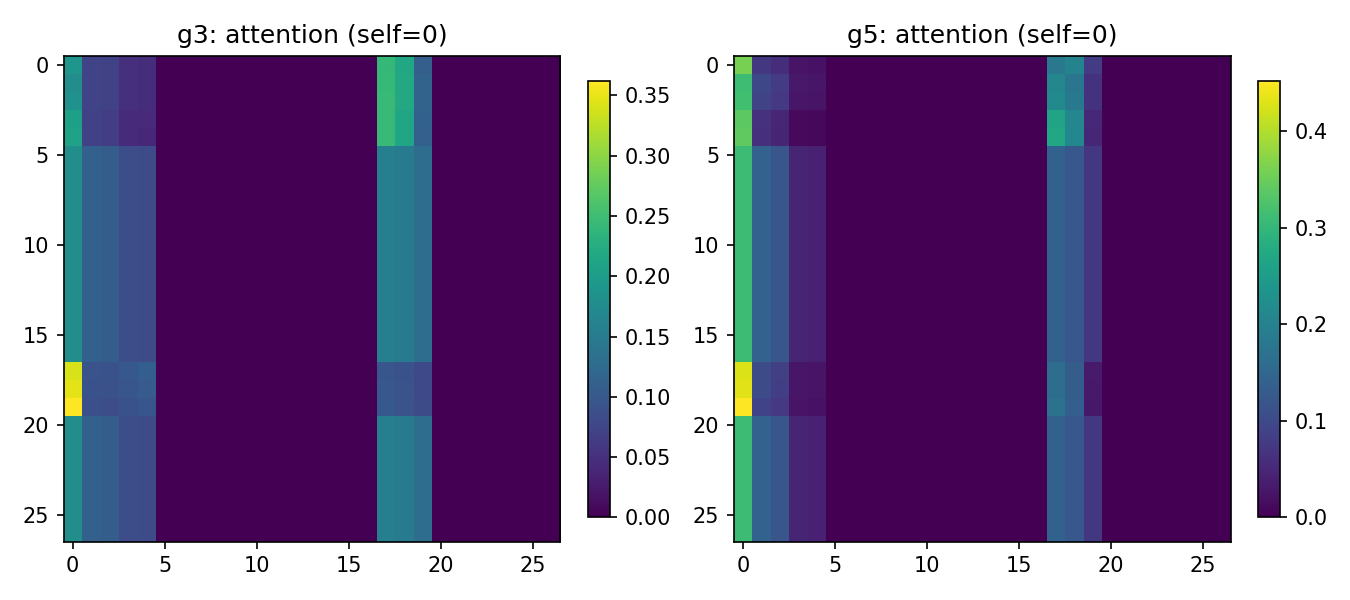
\includegraphics[width=0.9\linewidth]{../results/v3_1/saliency_v3.png}
\caption{Entity-attention weights for \giii{} (left) vs \gv{} (right),
sampled from the first agent after 30 warm-up steps. \giii{}'s attention
concentrates on a handful of entity slots (mostly nearby zombies);
\gv{}'s attention spreads more broadly, consistent with its need to
track knight lock targets as well as its own candidates.}
\label{fig:saliency}
\end{figure}

\subsection{Side-by-side demo}

A side-by-side video
(\texttt{results/v3\_1/demo\_sidebyside\_v3.mp4}) compares \gz{} (left,
heuristic) with \gv{} (right, learned) on seed 42. It illustrates the
qualitative difference between an unrestricted, high-fire-rate archer
that tries to cover the whole screen and a learned policy that uses
88\% of its ammo while respecting locks and the pragmatic override.

\section{Discussion}
\label{sec:discussion}

\subsection{The full curriculum matters}

Every coordination primitive contributes positively to the final score:

\[
\underbrace{\gii{} \to \giii{}}_{+2.30}\;
\underbrace{\giii{} \to \giv{}}_{+3.30}\;
\underbrace{\giv{} \to \gv{}}_{+3.80}
\]
in stochastic score. No primitive is redundant. The pragmatic override
(\gv{}) is the \emph{single largest} step, even though it only fires
when a zombie is projected to cross before a knight can intercept.

Intuitively, (i) roles prevent both knights from chasing the same
target, (ii) locks prevent archers from wasting arrows on zombies a
knight already owns, and (iii) the pragmatic override ensures that
respecting a lock does not cost the team a failure. Removing the
override (i.e.\ training \giv{} for 2 M steps instead of \gv{}) produces
a strictly worse policy on every metric we track.

\subsection{Deterministic results reinforce the structure story}

Under argmax, score climbs from strongly negative at \gii{}
($-1.90$) to strongly positive at \gv{} ($2.90$)---an absolute swing of
$+4.80$ along the progression. The intermediate step is noisier:
\giii{} deterministic ($0.60 \pm 1.43$) and \giv{} deterministic
($0.20 \pm 2.71$) differ by less than one standard error, so the pair
should be read as ``both approximately zero'' rather than as a
regression. The important signal is that by \gv{} the argmax mode is
substantively productive ($+2.90$, $\sigma = 2.62$), unlike the
constrained-but-stochastic failure pattern where argmax policies freeze
while sampling still fires. The transition \giv{} $\to$ \gv{}
(stochastic $+3.80$, deterministic $+2.70$) is the single largest step
on both metrics: the override turns a policy that was
committed-but-rigid (\giv{}, 0.2 deterministic) into one that is
committed and flexible (\gv{}, 2.9 deterministic).

\subsection{Peak is above the unrestricted ceiling}

\gv{}'s stochastic score (11.20) exceeds \gz{}'s (8.70) despite \gz{}
having no ammo cap, no stamina cost, and no role / lock rules. The
mechanism is ammo efficiency: \gz{} fires 306.8 attacks/episode for 7.5
archer kills (2.4\% hit rate), whereas \gv{} fires 56.7 attacks/episode
for 12.3 archer kills (21.7\% hit rate, 9$\times$ higher). The trained
archer waits for a high-probability shot; the heuristic empties the
clip at anything that moves.

\subsection{Failures as a live signal}

All seven games report $n_f \in [1.8, 3.0]$ failures per episode, so the
failure penalty $p_f \cdot \min(n_f^{(t)}, 3)$ is a live gradient at
training time. \gv{} \emph{minimises} failures (1.8) while
\emph{maximising} score (11.20). This is not a coincidence: the
pragmatic override exists exactly to prevent breaches, and its
quantitative payoff shows up on both sides of the score equation.

\subsection{Ammo-mode tie}

\ga{} and \gb{} produced almost identical stochastic scores
($1.70 \pm 3.00$ vs $1.60 \pm 2.76$). The orchestration script picked
\texttt{global} by a deterministic $\ge$ tiebreak, and
\gii--\gv{} are all trained under the 60-arrow shared pool. A separate
run under individual-pool ammo is a clean follow-up experiment; we do
not expect the primitive ordering (roles > locks > pragmatic) to
change, but the absolute scores could shift.

\section{Limitations and Future Work}
\label{sec:future}

\begin{enumerate}[nosep]
\item \textbf{Lock-radius sweep.} We chose $0.25\,W$ (320 px) based on a
  single run. A systematic sweep in $\{0.15, 0.20, 0.25, 0.30\}\,W$
  would characterise the sensitivity of the \giv{} $\to$ \gv{} gap to
  this parameter.
\item \textbf{Spawn-rate stress test.} Under our pressure settings the
  failure penalty fires but remains modest. Pushing \texttt{spawn\_rate}
  to $\{4, 6\}$ would test whether \gv{}'s pragmatic override degrades
  gracefully or falls off a cliff.
\item \textbf{Per-role heads.} Splitting the shared policy into per-role
  heads (shared trunk, two knight heads, one archer head) could remove
  the need for the role\_id observation feature and reduce
  parameter-sharing interference.
\item \textbf{Learned pragmatic override.} We hard-code the
  cross-vs-intercept calculation. Letting the archer's policy learn when
  to override may reveal richer coordination patterns.
\item \textbf{Individual-ammo ablation.} Rerun \gii--\gv{} under
  individual ammo to test sensitivity to the \ga/\gb{} tiebreak.
\end{enumerate}

\section{Conclusion}

We presented a seven-game ablation on PettingZoo KAZ that isolates four
coordination primitives and measures their individual contribution to
score, per-class kills, and attack budgets. Under matched spawn
pressure and per-episode seeds, the learned progression
\gii{} $\to$ \gv{} is monotonic in both stochastic and deterministic
evaluation, and the peak learned policy outperforms the unrestricted
heuristic ceiling by $+29\%$. The pragmatic override (\gv{}) contributes
the single largest step in the progression and is the only primitive
that simultaneously raises kills and lowers failures, evidence that it
performs a genuine offence / defence trade-off rather than a one-sided
improvement. The full implementation, training pipeline, evaluation
harness, and 70-episode video archive are available in the project
repository.

\bibliographystyle{plainnat}
\bibliography{references}

\end{document}
